\cs{need to make clear the diff btw objects meaning the concept/class and meaning an instance}
\cs{need to discuss problematic of standard evaluation procedure of CV models}

Objects, being members of many categories, can be called by many names (e.g.,\ a duck can be called \name{duck, bird, animal} etc.). 
In \langvis research (\lv), the choice of a particular name for an object is a ubiquitous problem---it underlies virtually all tasks that model how speakers use language to refer to objects in the world, such as image description, visual question answering, referring expression generation, etc. 
%
\lv methods are generally based on object detection or image classification models (or the visual features extracted from them) that were pre-trained towards predicting the single correct label of objects. 
The set of labels are often determined rather arbitrarily---it may contain very specific (e.g.,\ \name{goblet, gyromitra}) as well as "basic-level" labels (e.g., \name{bus}; cf.\ the label inventory of the ILSVRC challenges; \citealt{ILSVRC15}). 

This pre-training strategy has its justification in that computer vision models can learn rich, discriminative visual feature representations which capture fine-grained differences in object appearances (e.g.,\ sharp--pointed vs. slightly pointed). 
It is, however, different from predicting the natural name of an object, 
because, as has been found in numerous studies in psychology, humans have a preference towards a particular name (\textit{entry-level name}, e.g.,\ \name{duck}) when naturally calling an object  \cite{rosch1976basic,Rosch1978,jolicoeur1984pictures}. 
Entry-level names have hereby usually been considered to be an attribute of concrete \textit{concepts} (e.g.,\ penguin, duck), where the choice of a concept's entry-level name depends on factors such as its typicality with respect to its basic-level category (bird). \cs{Need to check Jolicoeur and their experiments} 
Crucially, though, as we will empirically show, human object naming is \textit{instance}-dependent---contextual visual features may humans have prefer different names for object instances of the same concrete concept, and have them even disagree in their choice for the same instance (see also \citealt{graf2016animal}). 
For example, Figure~\ref{fig:duck} shows two instances of the concept duck, and when people were asked to name the highlighted object, most ($27$) people called the instance on the left \name{bird}, while \name{duck} was strongly preferred for the right instance. 

Despite its relevance in \lv, the challenge of instance-based natural naming has been overseen, and most \lv datasets not necessarily provide enough information to make progress on the problem of modeling natural object naming (they only provide very few names). 
Research that particularly focuses on the prediction of entry-level names is scarce, and existing work has adopted the view that (i) entry-level names arise on the conceptual level, and (ii) developed specialized methods \cite{Ordonez:2016}. 
%To our knowledge, work that gives systematic insights into the ability of standard object recognition models to account for natural object naming, and in how far simple \cs{straightfoward?} re-training or transfer learning can increase this ability, is lacking. 
%
\begin{figure}
	\centering
	\small
	\begin{tabular}{p{3cm}p{3cm}}
		%VisualGenome+ManyNames & \cite{snodgrass}\\
		\centering
		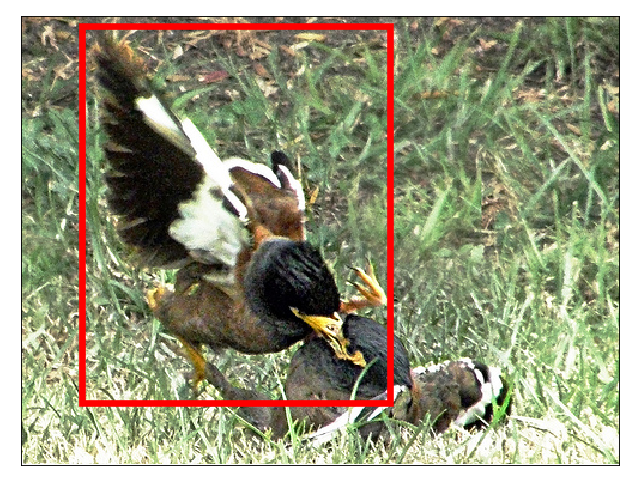
\includegraphics[scale=0.15]{images/2327551_2960743_seed_ambiguous.png} &
		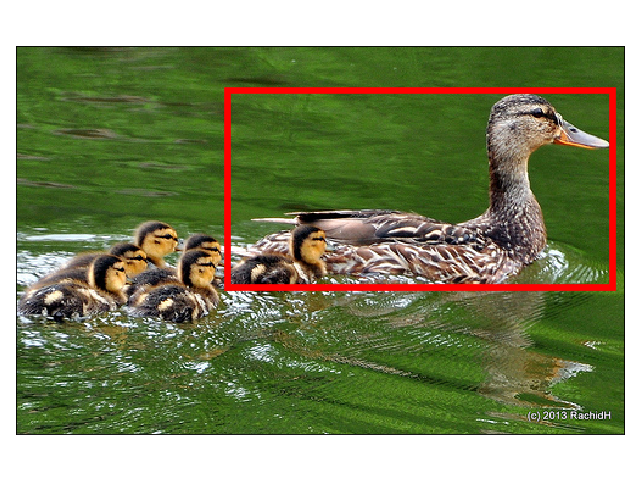
\includegraphics[scale=0.15]{images/2358126_805887_singleton_obj.png}\\
		bird\ (27),  duck\ (8) & duck (33), bird (3)\\
	\end{tabular}
	
	\caption{Different naming preferences for different instances of the same concept (duck)\label{fig:duck}}
\end{figure}
%
In this paper, we seek an understanding of the notion of entry-level names of instances of real-world objects in images, and to give systematic insights into the problem of retraining or fine-tuning object detection models (and features in transfer learning) such that they capture a natural vocabulary and account for linguistic preferences in naming. %, i.e.,\ the name that humans naturally prefer to call an object.  
Specifically, and in contrast to previous works, we 
(i) take on an empirical notion of entry-level names, and define it on the instance-level, i.e., the name that humans prefer to use when calling a particular object in a real-world image.   
(ii) We examine in how far standard models in computer vision, namely object detection and image classification models, do learn entry-level naming by being trained on images labeled with rather \textit{\arbitrary} (as opposed to entry-level) object names. \cs{add sth based on results - how to fine-tune or whether it's possible to fine-tune; how readily available they are to be used for transfer learning, the standard method in \lv}

We use \mn, a new dataset of real-world images, built on top of \vg, which provides an excellent resource for our study, since it was annotated with a large number\ $(36)$ of object names by means of a crowdsourcing study.

Our contributions are: 
(i) We present our extension of the \mn dataset that augments all collected object names with verification information, which allows an in-depth analysis of naming models on the task of object naming. 
(ii) Theoretical:
(a) We show that entry-level names should be derived on the instance-level as opposed to the XXX level \cs{(TO SHOW: entry-level names are different for the same "class" @Sina or @Matthijs?) (contrast to psychological studies)}
(b) We need many name annotations to derive the entry-level name (contrast to few annotations in L+V and computer vision; \cs{TO SHOW: entry-level name of an instance varies depending on the number of annotations/instance)}
(iii) Technical:
(a) Object detectors trained on "\arbitrary" natural object names do learn entry-level names to some extend (as expected: they learn the shared features leading to entry-level \cs{-- can we show that mistakes are rather class-based? i.e., tendency towards a certain name for each class?)}
(b) To predict entry-level names without annotating a huge amount of training examples, it is possible to fine-tune (iii) on \mn. We show that \cs{(say something about mistakes not made anymore). }

